\section{Goals and Assumptions}\label{s:deploy}
\begin{figure*}[t]
    \centering
    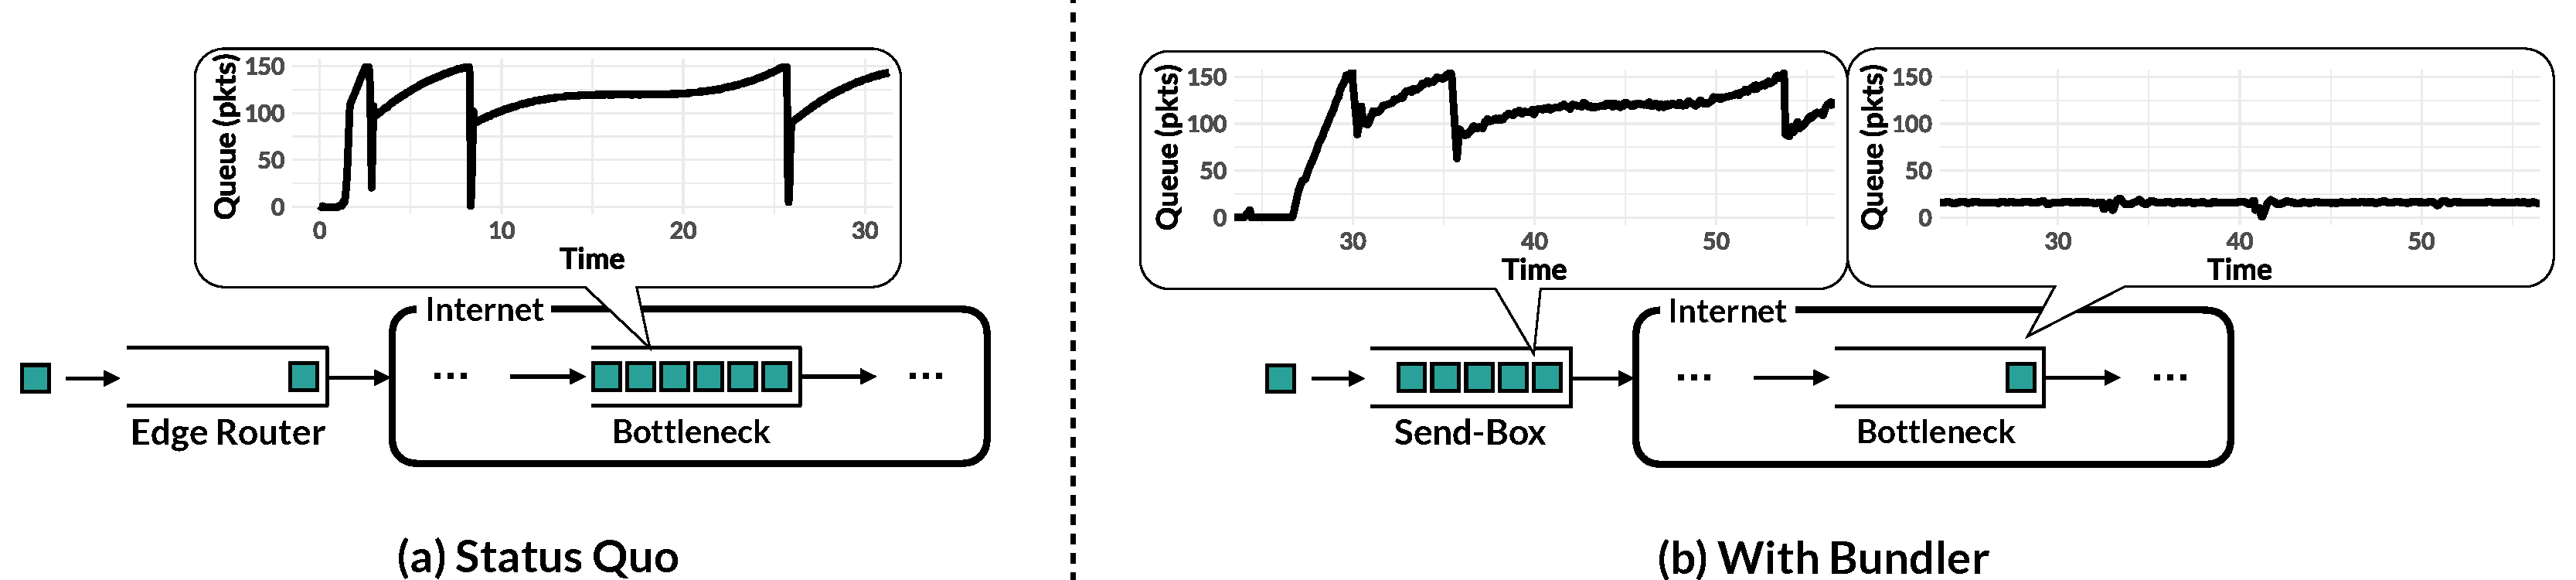
\includegraphics[width=\textwidth]{img/shift-bottleneck-combined}
    \caption{This illustrative example with a single flow shows how \name can take control of queues in the network. The plots, from measurements on an emulated path (as in \S\ref{s:eval}), show the trend in queueing delays at each queue over time. The queue where delays build up is best for scheduling decisions, since it has the most choice between packets to send next. Therefore, the \inbox \emph{shifts} the queues to itself.}\label{fig:design:shift-bottleneck}
\end{figure*}
%

%\fc{Would it be better to lead with some example of how theres a large amount of traffic bewteen A and B? }

%%\radhika{add more examples}
%%
%%\radhika{Add a new section on ``Requirements/Assumptions'' here that has the text below}
%%
%%\cut{
%%\Para{Amount of Aggregation} 
%%A traffic bundle, to be useful, must be \emph{heavyweight} enough to drive self-inflicted queueing in the network; these queues, once under \name's control, provide scheduling opportunities. We expect many bundles to be heavyweight in practice because a majority of Internet traffic today is owned by a few large content providers who host a wide array of services~\cite{fivecomps, labovitz}. 
%%}

Figure~\ref{fig:deploy:arch} describes \name's deployment model. 
\name aggregates traffic from Site A to Site B, and vice-versa, into two unidirectional bundles. 
In the egress path, the \inbox moves the in-network queues built by the bundled traffic to itself (illustrated in Figure~\ref{fig:design:shift-bottleneck}) (we describe the specific mechanism in \S\ref{s:design}). 
It can thus enforce desired scheduling policies across the traffic in the bundle.

Our primary goal with \name is to provide control over \emph{self-inflicted} queueing, \ie when traffic from a single bundle causes a queue to build up at the bottleneck links in the network, even without any other cross-traffic.
%cases when traffic within the same bundle should be reordered according to the site administrator's policy.
In the remainder of this section, we detail the conditions in which \name can achieve this goal. Our high-level strategy is ``do no harm''; \name detects conditions in which it cannot operate and temporarily disables itself until favorable conditions return, reverting to status-quo performance in the meantime.
%\radhika{read again after intro has been written}

\Para{Non-edge bottleneck}
Network administrators already have control over packets which queue within their site. \name is capable of taking control over queues that build up anywhere between a \pair. Thus, deploying \name at the edge of each site captures any potential build up outside of either site's control. Such congestion might occur at an inter-domain link, within either site's ISP, or, if a site is managed by a cloud provider, it could even occur within its datacenter (\eg{} at the cloud provider's rate limiter, \S\ref{s:eval:realworld}). 
% \name is thus useful for moving queues that build up due to congestion in the ``middle'' of the network (\ie \emph{anywhere} along the path between a \pair). 

There is strong evidence that such non-edge bottlenecks exist.
Dhamdhere \etal measured~\cite{inferring-interdomain-congestion} inter-domain bottlenecks such as the red bottleneck link in Figure~\ref{fig:deploy:arch}, and
Zhu \etal found~\cite{bottleneck-of-china} that non-edge bottlenecks for transnational traffic to and from China are prevalent, and moreover that in many cases, the bottleneck for this traffic is an ISP deep inside China rather than a larger provider.
An M-Lab technical report similarly found~\cite{mlab-tr} patterns of performance degradation linked to specific ISP interconnections in the middle of the network.
Finally, Jin \etal found~\cite{blameit} that for for WAN traffic originating from Microsoft Azure, the ``middle'', \ie on-path ASes not including the source or destination AS, is to blame for between $40$-$50\%$ of persistent congestion incidents over a one-month period. 

\Para{External congestion} Other than self-inflicted congestion, \name must coexist with traffic from external sources.
%It can happen when a small carrier network does not have enough capacity to sustain the large volume of traffic sent by a content provider to a receiving domain, or due to explicit rate limiting commonly done by ISPs~\cite{isp-throttle-1, isp-throttle-2, isp-throttle-3}. 
%In such cases, \name can result in significant improvements in performance, as it would then have control over the entire queue. 
%In our experiments (\S\ref{s:eval}), we found this to be the case.

\vspace{2pt}
\paragraphi{Congestion due to bundled cross-traffic}
%In-network congestion can further increase in the presence of other cross-traffic (\eg when the peering link between Carrier 2 and the enterprise in Figure~\ref{fig:deploy:arch} is shared by traffic from multiple content providers' domains). 
\name continues to provide benefits when the competing flows are part of other bundles from/to other sites because the rate control algorithm at each of the other {\inbox}es would ensure that the in-network queues remain small, and different bundles compete fairly with one another. Since each \inbox manages the self-inflicted queues for its own bundles, it can apply the appropriate scheduling policy in its per-bundle queues.
%\fc{X?->}We expect this to become the common form of observed congestion as more sites deploy \name. 

\vspace{2pt}
\paragraphi{Congestion due to un-bundled cross-traffic} We now consider the scenario where the cross-traffic includes un-bundled flows. If all such \emph{un-bundled} competing flows are short-lived (up to a few MBs) or application-limited (\eg a paced video stream), the bundled traffic still sees significant performance benefits, because there are not enough packets in such short-lived flows to fill up the queues or claim a greater share of network bandwidth.
%\radhika{Likewise, \name continues to provide performance benefits in the presence long-lived rate-controlled cross-traffic (e.g. a paced video stream) that also does not fill up queues.} 
However, if the cross traffic is long lasting, and employs a loss-based congestion controller to send back-logged bulk data, it aggressively fills up all available buffer space at the bottleneck link. Naively using a delay-based congestion controller at \name against such aggressive \emph{buffer-filling} cross-traffic would severely degrade the throughput of the bundled traffic. Therefore, \name's congestion controller detects the presence of buffer-filling cross-traffic;
% to compete fairly, pushes more packets into the network. 
to compete fairly, it relinquishes most of its control (and scheduling opportunities) over the bundled traffic, while still maintaining a small queue for continued detection of cross-traffic (detailed in \S\ref{s:buffer-filling}). 
%\radhika{cut:/*} This extra queueing results in a slight latency increase that we evaluate in \S\ref{s:robust:cross}.\radhika{*/}
%However, in these cases, \name chooses to create extra queueing as described in \S\ref{s:queue-ctl} to be able to detect when the cross traffic leaves.
%Therefore, the bundle's aggregate throughput will decrease slightly due to RTT unfairness.
%We evaluate this phenomenon in \S\ref{s:robust:cross}.
%\radhika{Maybe add: ``Note that not all long-lasting flows are detected as buffer-filling (e.g. a video stream that sends paced packets does not fill buffers). A pathological buffer-filling flow is both long-lasting and comprises of a backlogged bulk transfer.}
However, such pathological buffer-filling cross traffic is rare.
%\radhika{cut:/*} To understand why, consider that cross traffic must be (a) bottlenecked at the same link as the bundle traffic and (b) long-lived enough to build persistent queues.\radhika{*/}
A recent study in CDNs~\cite{akamai-cdn-trace} and our analysis of a packet trace from an Internet backbone router~\cite{caida-dataset} reveal that the vast majority of connections are smaller than 1MB: too small to build persistent queues.\footnote{\cut{\radhika{check:} }This implies that flows \emph{within} a bundle may also be short-lived requests or paced audio/video traffic which, when aggregated by \name, can form a heavy, long-lasting bundle.} 
%\radhika{One might ask that given long-lasting flows are rare, how can \name do effective rate control. Should we add a footnote or a line that says ``Even the components of a bundle are likely to be short-lived flows (up to a few MBs) \fc{+1} and paced audio/video traffic that arrive at different times, creating a heavy long-lasting bundle on an aggregate.''} 
Our experiments on Internet paths (\S\ref{s:eval:realworld}), also did not encounter pathological buffer-filling cross traffic.  

%\radhika{Akshay, check this out.}
%We further analyze a packet trace from an Internet backbone router~\cite{caida-dataset}.
%The flow size distribution here is even more skewed: $97.6\%$ of flows are under $10$KB, and only $0.02\%$ of flows are larger than $5$MB.

\Para{Shared congestion across flows in the bundle} Bundler’s design for moving queues via aggregate congestion control assumes that the component flows within a bundle share in-network paths, and thus congestion. 
%\an{I am mentioning the traceroute measurements here:} 
To test this assumption, we used Scamper~\cite{scamper} to probe all paths to $5000$ random IPv4 addresses from each of $30$ cloud instances across the regions of public cloud providers AWS and Azure. In no cases did we find that probe packets took different AS-level paths through the network.
%\an{be careful about persistent imbalance claim}
%Of course, IP-level load balancing exists, and we detect it. 
However, we observed instances of IP-level load balancing in 26\% of IP hops. 
In pathological scenarios with \emph{persistent imbalance} in queueing between the load-balanced paths, \name cannot gather accurate measurements and perform aggregated delay-based rate control for the bundled traffic. 
Designing a new congestion control algorithm for such scenarios remains an avenue for future work.
Nonetheless, \name can detect these scenarios (\S\ref{s:queue-ctl:ecmp}) and disable its rate control in such cases, falling back to status-quo performance. 
We expect a well-implemented load balancer will work to prevent persistent imbalance from occurring; indeed, our success with using \name on real Internet paths (\S\ref{s:eval:realworld}) suggests that such pathological cases do not occur in practice.
%\radhika{cut:/*}Transient imbalance may be common. In these cases, \name's congestion controller, which uses a simple delay control law (\S\ref{s:design:whichcc}), may fluctuate its rate in response to measurements of the different queues. \name's control over the queue will thus fluctuate, but it can still provide scheduling benefits. \radhika{*/ we don't have results for this, right? readers may not get what we are saying at this point anyway} 
%\fc{did we intentionally remove the assumption about having "enough" traffic? i know it's fairly "obvious" but might be good to have at least one sentence clarifying this somewhere.} \radhika{i am fine with adding it back in. although, we might be saying something to that effect in the intro already.}
%Designing a new congestion control algorithm for this scenario remains an avenue for future work.
%Another common scenario is for the bottleneck to be at the edge of the receiving domain, which will again be shared across the bundled flows. Finally, even if an in-network load balancing mechanism splits the bundled flows across multiple congested paths with multiple in-network queues, \name would account for the aggregate network bandwidth and move all of these queues to the sender's domain. 

%(2) from the bundle's perspective, multiple paths appear as multiple queues, with some aggregate bandwidth capacity (\ie the max-flow of the network paths between the sending and receiving domains). While queueing may be unevenly distributed among the paths, the distribution of flows onto paths is currently random (\eg via ECMP). With \name, all these queues are moved to the \inbox, so it can schedule bundled flows deliberately rather than randomly.

\paragrapha{Intuition for \name's applicability}
Another way of understanding when \name is useful, which incorporates the three conditions above, is the following litmus test:
compare the queueing delay when all flows (\name's and cross-traffic) are in the network with the queueing delay when the \name’s flows are magically removed; if the latter is lower than the former, then \name can provide benefits.

\cut{
\vspace{0.05in}
\paragrapha{Takeaway} While \name must yield its scheduling ability in the face of aggressive, buffer-filling cross traffic and persistently imbalanced load balancing, in most scenarios it significantly improves performance (as we show in \S\ref{s:eval}).
This, combined with its deployment ease, makes a strong case for deploying \name. 
}
